\section{Definizione di remote sensing}
Il \textbf{remote sensing} (o telerilevamento) \cite{ALL1_REMOTE_SENSING, ALL2_REMOTE_SENSING,
ALL3_REMOTE_SENSING, ALL4_REMOTE_SENSING, ALL5_REMOTE_SENSING}  è la disciplina 
tecnico-scientifica che si occupa di acquisire informazioni di 
carattere spettrale, spaziale e temporale su 
oggetti materiali, su una determinata area o relativamente ad uno 
specifico fenomeno, senza avere contatto fisico con l’oggetto di 
studio, o con il fenomeno in esame. 
Il telerilevamento è, dunque, la misurazione o l'acquisizione di 
informazioni di alcune proprietà di un oggetto o fenomeno, da un 
dispositivo di registrazione che non è in contatto con l'oggetto o il 
fenomeno in esame.
I dispositivi che vengono utilizzati in questo ambito sono diversi: 
fotocamere, laser e ricevitori a radiofrequenza, sistemi radar.  

% Questa tecnologia è ampiamente impiegata nell’ osservazione della superficie 
% terrestre. Nello svolgimento di tale attività i sensori sono posti a quote elevate in 
% modo tale da poter acquisire immagini di aree molto vaste. I sensori non usano solo 
% la luce visibile ma operano anche mediante altre bande dello spettro 
% elettromagnetico {(Figura \ref{fig:BandeSpettroElettromagnetico})}  come infrarossi, microonde e ultravioletto.

Negli ultimi decenni il telerilevamento ha subito degli sviluppi tali da essere, 
oggigiorno, uno strumento fondamentale per la raccolta di informazioni su quasi 
ogni aspetto della terra.  
Il telerilevamento trova applicazione in numerosi contesti accomunati 
dalla necessità di acquisire dati relativi ad aree molto estese. 
Tra le principali applicazioni si includono:
\begin{itemize}
    \item Mappatura e analisi dell'uso del suolo;
    \item Monitoraggio della vegetazione in ambito agricolo e forestale;
    \item Monitoraggio delle risorse idriche, della neve e del ghiaccio;
    \item Indagini archeologiche;
    \item Gestione di eventi calamitosi;
    \item Gestione delle risorse costiere \cite{ALL3_REMOTE_SENSING, Descrizione_Piattaforme}.
\end{itemize}

% Il telerilevamento può trovare applicazione in numerosi contesti , accomunati 
% dalla necessità di acquisire dati relativi ad un’area molto estesa. Attualmente tra le 
% applicazioni del telerilevamento si ha la mappatura e l’analisi dell'uso del suolo, il 
% monitoraggio della vegetazione in ambito agricolo e forestale, il monitoraggio delle 
% risorse idriche, della neve e del ghiaccio, della fauna selvatica, le indagini 
% archeologiche, la gestione di eventi calamitosi, la gestione delle risorse costiere, 
% applicazioni in ambito militare e molte altre. 



Ogni applicazione ha necessità di sensori con caratteristiche tecniche differenti, con 
specifiche capacità di risoluzione spettrale, risoluzione spaziale, risoluzione 
radiometrica e risoluzione temporale. Inoltre, i sistemi di telerilevamento possono 
fornire dati e informazioni in aree in cui l'accesso è difficile a causa della 
conformazione del terreno o delle condizioni meteorologiche \cite{GISGeography_RemoteSensing}.  


Nel telerilevamento è inoltre compresa anche l'analisi e l'interpretazione di dati e 
immagini. Questo aspetto è fondamentale in quanto per poter cogliere le 
informazioni chiave per l’obiettivo che si sta perseguendo bisogna avere buona 
comprensione della base fisica e del processo di acquisizione, nonché di una solida 
conoscenza degli algoritmi utilizzati per elaborare i dati.

I dati vengono acquisiti dai sensori, i quali devono essere installati su specifiche 
piattaforme, mezzi o veicoli. Droni, aerei e satelliti raccolgono la maggior parte dei 
dati ma molti di questi strumenti possono essere installati anche su piattaforme 
terrestri, come autocarri e trattori.  

\subsection{Piattaforme di Telerilevamento}

I dati di telerilevamento vengono acquisiti da sensori installati su 
piattaforme specifiche, che si classificano in tre categorie 
principali \cite{Rappresentazione_piattaforme, Descrizione_Piattaforme}:


\begin{itemize}
    \item \textbf{Spaceborne}: Satelliti come Sentinel-2 offrono dati a bassa risoluzione ma un'ampia copertura spaziale \cite{Munich480}.
    \item \textbf{Airborne}: UAV (Unmanned Aerial Vehicle) e aerei più versatili, consentono acquisizioni ad alta risoluzione spaziale.
    \item \textbf{Ground-based}: Dispositivi a terra forniscono dati ad altissima risoluzione per dettagli locali.
\end{itemize}

\begin{figure}[H]
    \centering
    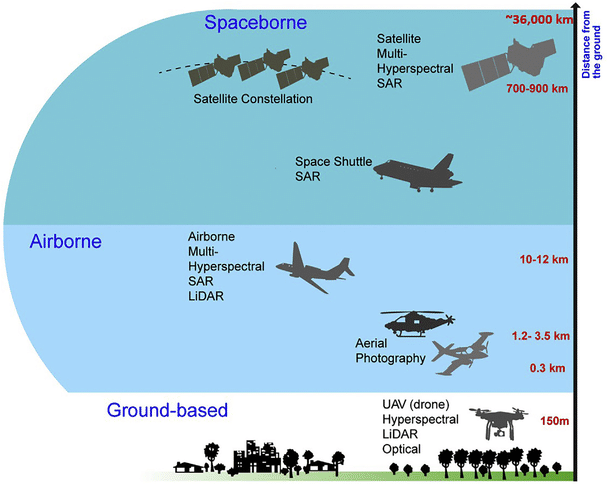
\includegraphics[width=0.7\textwidth]{Immagini/Generiche/Common-Remote-Sensing-Platform-a.png}
    \caption{Rappresentazione delle piattaforme \cite{Rappresentazione_piattaforme}.}
    \label{fig:Classificazione_Piattaforme}
    %Figura 2.1: Esempio schematico di un neurone
\end{figure}


